\textbf{Un pescador est\'a sobre un oc\'eano rectangular. El valor del pez en el punto $(i, j)$ est\'a dado por un arreglo A de dimensi\'on 2 $n \times m$. Dise\~na un algoritmo que calcule el m\'aximo valor de pescado que un pescador puede atrapar en un camino desde la esquina superior izquierda a la esquina inferior derecha. El pescador solo puede moverse hacia abajo o hacia la derecha, como se ilustra en la siguiente figura.}\vspace{.2cm}

\begin{figure}[H]
    \centering
    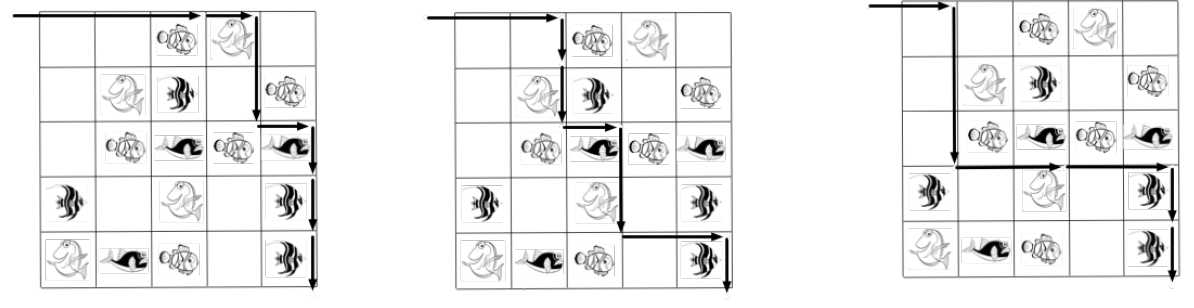
\includegraphics[width=0.75\linewidth]{src/Img/lago.PNG}
\end{figure}

Como en basicamente toda la tarea, vamos a usar programacion dinamica. El punto es calcular el maximo valor de pescado que se puede atrapar en un camino desde la esquina superior izquierda a la esquina inferior derecha. Ademas, solo vamos a considerar los movimientos hacia abajo y hacia la derecha. (uno a la vez). \vspace{.2cm}

\textbf{Nota:} Voy a asumir que la matriz tiene al menos una fila y una columna, si no, no tiene sentido, ademas no voy a considerar que un pez pueda tener valor negativo aunque me parece no afecta al algoritmo. \vspace{.2cm}

\textcolor{bibi}{Programación dinámica:} \vspace{.2cm}
\begin{quote}
    De hecho este problema se parece bastante a la subcadena mas larga, en este caso ya tenemos el arreglo auxiliar y le vamos a meter informacion a las celdas, lo podemos hacer poniendole un valor de valorM o algo por el estilo. (podemos usar otra matriz con las mismas dimensiones tambien) \vspace{.2cm}

    Empezando por caracterizar el problema, vemos que el pescador solo puede llegar a la celda (i,j) si antes estuvo en la celda (i-1,j) o en la celda (i,j-1). Por lo tanto, el valor en la celda (i,j) se puede entender como el valor del pez en esa celda mas el maximo valor entre las 2 que puede llegar. Ademas, el pescador siempre empieza en la celda (0,0) por tanto esta celda solo sera el valor del pez que haya o no ahi. \vspace{.2cm}

    Entonces la funcion de recurrencia es la siguiente: (estamos guardando valorM por celda) \vspace{.2cm}
    \begin{align*}
        valorM[i][j]=\begin{cases}
            valorPez[0,0] & \text{si } i=0 \text{ y } j=0 \\
            valorM[0][j-1]+valorPez[0,j] & \text{si } i=0 \\
            valorM[i-1][0]+valorPez[i,0] & \text{si } j=0 \\
            max(valorM[i-1][j],valorM[i][j-1])+valorPez[i,j] & \text{si } i>0 \text{ y } j>0
        \end{cases}
    \end{align*}

    Entonces comenzamos a llenar la matriz, primero la celda (0,0) sera el valor del pez en esa celda. Despues llenamos la primera fila y la primera columna con la recurrencia que pusimos arriba. Finalmente llenamos el resto de la matriz con la recurrencia y al final el valor que buscamos es el valor en la celda (n-1,m-1). \vspace{.2cm}

    Veamos un ejemplo: \vspace{.2cm}

    \begin{table}[H]
        \centering
        \begin{tabular}{|l|l|l|l|l|l|}
            \hline
            \textit{{[}5,*{]}} & \textit{{[}0,*{]}} & \textit{{[}0,*{]}} & \textit{{[}8,*{]}}                         & \textit{{[}4,*{]}}                         & \textit{{[}2,*{]}}                         \\ \hline
            \textit{{[}1,*{]}} & \textit{{[}2,*{]}} & \textit{{[}3,*{]}} & \textit{{[}0,*{]}}                         & \textit{{[}0,*{]}}                         & \textit{{[}7,*{]}}                         \\ \hline
            \textit{{[}5,*{]}} & \textit{{[}1,*{]}} & \textit{{[}0,*{]}} & \textit{{[}0,*{]}}                         & \textit{{[}3,*{]}}                         & \textit{{[}6,*{]}}                         \\ \hline
            \textit{{[}6,*{]}} & \textit{{[}0,*{]}} & \textit{{[}0,*{]}} & \cellcolor[HTML]{FFFFFF}\textit{{[}9,*{]}} & \cellcolor[HTML]{FFFFFF}\textit{{[}1,*{]}} & \cellcolor[HTML]{FFFFFF}\textit{{[}1,*{]}} \\ \hline
        \end{tabular}
    \end{table}

    Aqui, comenzamos con un arreglo A de dimension 6x4, cada celda puede o no tener un pez con un valor asociado, ademas, simbolice [valorPez,valorM] siendo que no hemos calculado ningun valorM, esta como * para indicar que no lo hemos calculado. \vspace{.2cm}

    Empezamos sabiendo que el valor en la celda (0,0) es 5, y de ahi usamos los 2 primeros casos para llenar la primera fila y la primera columna. \vspace{.2cm}
    \begin{table}[H]
        \centering
        \begin{tabular}{|l|l|l|l|l|l|}
            \hline
            \textit{{[}5,5{]}}  & \textit{{[}0,5{]}} & \textit{{[}0,5{]}} & \textit{{[}8,13{]}}                        & \textit{{[}4,17{]}}                        & \textit{{[}2,19{]}}                        \\ \hline
            \textit{{[}1,6{]}}  & \textit{{[}2,*{]}} & \textit{{[}3,*{]}} & \textit{{[}0,*{]}}                         & \textit{{[}0,*{]}}                         & \textit{{[}7,*{]}}                         \\ \hline
            \textit{{[}5,11{]}} & \textit{{[}1,*{]}} & \textit{{[}0,*{]}} & \textit{{[}0,*{]}}                         & \textit{{[}3,*{]}}                         & \textit{{[}6,*{]}}                         \\ \hline
            \textit{{[}6,17{]}} & \textit{{[}0,*{]}} & \textit{{[}0,*{]}} & \cellcolor[HTML]{FFFFFF}\textit{{[}9,*{]}} & \cellcolor[HTML]{FFFFFF}\textit{{[}1,*{]}} & \cellcolor[HTML]{FFFFFF}\textit{{[}1,*{]}} \\ \hline
        \end{tabular}
    \end{table}

    Ahora toca lo interesante, utilizar el tercer caso para llenar el resto de la matriz. \vspace{.2cm}

    \begin{table}[H]
        \centering
        \begin{tabular}{|l|l|l|l|l|l|}
            \hline
            \textit{[5,5]}  & \textit{[0,5]}  & \textit{[0,5]}  & \textit{[8,13]}                         & \textit{[4,17]}                         & \textit{[2,19]}                         \\ \hline
            \textit{[1,6]}  & \textit{[2,8]}  & \textit{[3,11]} & \textit{[0,13]}                         & \textit{[0,17]}                         & \textit{[7,26]}                         \\ \hline
            \textit{[5,11]} & \textit{[1,12]} & \textit{[0,12]} & \textit{[0,13]}                         & \textit{[3,20]}                         & \textit{[6,32]}                         \\ \hline
            \textit{[6,17]} & \textit{[0,17]} & \textit{[0,17]} & \cellcolor[HTML]{FFFFFF}\textit{[9,26]} & \cellcolor[HTML]{FFFFFF}\textit{[1,27]} & \cellcolor[HTML]{FFFFFF}\textit{[1,33]} \\ \hline
            \end{tabular}
    \end{table}

    Realmente el proceso aun manual es bastante facil solo es sumar el valor del pez en esa posicion mas el maximo valor que puede llevar de arriba o de la izquierda, en este caso el maximo total que puede conseguir es 33, y mas aun podemos recuperar el camino viendo desde que lado vino: \vspace{.2cm}

    \begin{table}[H]
        \centering
        \begin{tabular}{|l|l|l|l|l|l|}
            \hline
            \rowcolor[HTML]{FFFC9E} 
            \textit{[5,5]}  & \textit{[0,5]}  & \textit{[0,5]}  & \textit{[8,13]}                         & \textit{[4,17]}                         & \textit{[2,19]}                         \\ \hline
            \textit{[1,6]}  & \textit{[2,8]}  & \textit{[3,11]} & \textit{[0,13]}                         & \textit{[0,17]}                         & \cellcolor[HTML]{FFFC9E}\textit{[7,26]} \\ \hline
            \textit{[5,11]} & \textit{[1,12]} & \textit{[0,12]} & \textit{[0,13]}                         & \textit{[3,20]}                         & \cellcolor[HTML]{FFFC9E}\textit{[6,32]} \\ \hline
            \textit{[6,17]} & \textit{[0,17]} & \textit{[0,17]} & \cellcolor[HTML]{FFFFFF}\textit{[9,26]} & \cellcolor[HTML]{FFFFFF}\textit{[1,27]} & \cellcolor[HTML]{FFFC9E}\textit{[1,33]} \\ \hline
        \end{tabular}
    \end{table}

    La complejidad de este algoritmo es de $O(n*m)$ y usa $O(n*m)$ memoria (es equivalente agregar un valor por cada valor a usar otro arreglo pero asi se ve mas bonito uwu), esto pues la matriz es de tamaño $n*m$ y se llena en cada celda una vez tomando $O(1)$ tiempo (checar arriba y abajo, tomar un indice de un arreglo). \vspace{.2cm}
\end{quote}